% =============================================================================
% relatorio_crc.tex -- Relatorio Tecnico: CRCChip v1.0
% Unidade 7 | Capitulo 5 | Desafio de Design de CIs -- PADIS
% Autor  : Pedro Victor dos Santos Oliveira
% Prof.  : Thiago Brito
% =============================================================================
\documentclass[12pt,a4paper]{article}

\usepackage[utf8]{inputenc}
\usepackage[T1]{fontenc}
\usepackage[brazil]{babel}
\usepackage{lmodern}
\usepackage{microtype}
\usepackage{geometry}
% Margens ABNT (NBR 14724)
\geometry{top=3cm,bottom=2cm,left=3cm,right=2cm}
\usepackage{setspace}
\onehalfspacing
\usepackage{graphicx}
\usepackage[dvipsnames,table]{xcolor}
\usepackage{tikz}
\usetikzlibrary{shapes.geometric,arrows.meta,positioning,fit,calc,shadows,decorations.pathreplacing}
\usepackage{pgfplots}
\pgfplotsset{compat=1.18}
\usepackage{booktabs,multirow,array,longtable,colortbl}
\usepackage{listings,caption,subcaption}
\usepackage{amsmath,amssymb,mathtools,bm}
\usepackage{fancyhdr,titlesec,setspace,parskip,enumitem}
\usepackage[most]{tcolorbox}
\tcbuselibrary{listings,breakable,skins}
\usepackage[hidelinks,pdftitle={CRCChip v1.0},pdfauthor={Pedro Victor dos Santos Oliveira}]{hyperref}
\usepackage{siunitx}
\sisetup{output-decimal-marker={,},group-separator={.}}

% ── Cores ────────────────────────────────────────────────────────────────────
\definecolor{crcblue}{RGB}{21,101,192}
\definecolor{crcteal}{RGB}{0,137,123}
\definecolor{crcred}{RGB}{198,40,40}
\definecolor{crcgreen}{RGB}{46,125,50}
\definecolor{crcorange}{RGB}{239,108,0}
\definecolor{crcgray}{RGB}{66,66,66}
\definecolor{crcbg}{RGB}{245,248,252}
\definecolor{crccode}{RGB}{248,248,248}

% ── Listagem SV ──────────────────────────────────────────────────────────────
\lstdefinelanguage{SystemVerilog}{
  morekeywords={module,endmodule,input,output,logic,wire,reg,always_comb,
    assign,begin,end,case,endcase,default,if,else,parameter,localparam,
    task,endtask,automatic,initial,$dumpfile,$dumpvars,$display,$finish,int,
    timescale,string,genvar,generate,endgenerate},
  sensitive=true,
  morecomment=[l]{//},
  morestring=[b]",
}
\lstdefinestyle{svstyle}{
  language=SystemVerilog,
  basicstyle=\ttfamily\small,
  keywordstyle=\color{crcblue}\bfseries,
  commentstyle=\color{crcgray}\itshape,
  numbers=left, numberstyle=\tiny\color{crcgray}, stepnumber=1, numbersep=8pt,
  frame=single, framerule=0.6pt, rulecolor=\color{crcblue!40},
  backgroundcolor=\color{crccode},
  breaklines=true, showstringspaces=false, tabsize=4, captionpos=b,
  xleftmargin=15pt, xrightmargin=5pt,
}

% ── Caixas ───────────────────────────────────────────────────────────────────
\newtcolorbox{unidadebox}[1][]{enhanced,colback=crcbg,colframe=crcblue,
  coltitle=white,fonttitle=\bfseries\normalsize,title={#1},boxrule=1.2pt,
  arc=4pt,left=8pt,right=8pt,top=6pt,bottom=6pt,
  shadow={2pt}{-2pt}{0pt}{black!20},breakable}
\newtcolorbox{resultbox}[1][]{enhanced,colback=crcgreen!5,
  colframe=crcgreen!70!black,coltitle=white,fonttitle=\bfseries\small,
  title={#1},boxrule=1pt,arc=3pt,left=6pt,right=6pt,top=5pt,bottom=5pt,breakable}
\newtcolorbox{specbox}[1][]{enhanced,colback=crcblue!5,colframe=crcblue!60,
  coltitle=crcblue!80!black,fonttitle=\bfseries\small,title={#1},
  boxrule=0.8pt,arc=3pt,left=6pt,right=6pt,top=5pt,bottom=5pt,breakable}

% ── Cabecalho ────────────────────────────────────────────────────────────────
\pagestyle{fancy}\fancyhf{}
\fancyhead[L]{\small\textcolor{crcblue}{\textbf{CRCChip v1.0}}}
\fancyhead[C]{\small\textcolor{crcgray}{PADIS --- Unidade~7 / Capítulo~5}}
\fancyhead[R]{\small\textcolor{crcgray}{CRC-8/SMBUS}}
\fancyfoot[L]{\small\textcolor{crcgray}{Pedro Victor dos Santos Oliveira}}
\fancyfoot[C]{\small\textcolor{crcgray}{\thepage}}
\fancyfoot[R]{\small\textcolor{crcgray}{Prof.\ Thiago Brito}}
\renewcommand{\headrulewidth}{0.4pt}
\renewcommand{\footrulewidth}{0.4pt}

\titleformat{\section}{\large\bfseries\color{crcblue}}{}{0em}
  {\thesection.~}{}
\titleformat{\subsection}{\normalsize\bfseries\color{crcteal}}{}{0em}
  {\thesubsection.~}{}
\titleformat{\subsubsection}{\normalsize\bfseries\color{crcgray}}{}{0em}
  {\thesubsubsection.~}{}

% ── Resumo / Abstract env ────────────────────────────────────────────────────
\newenvironment{resumoenv}{%
  \begin{center}\textbf{Resumo}\end{center}\small\setlength{\parindent}{0pt}}{}
\newenvironment{abstractenv}{%
  \begin{center}\textbf{Abstract}\end{center}\small\setlength{\parindent}{0pt}}{}

% =============================================================================
\begin{document}
% =============================================================================

% ── CAPA ─────────────────────────────────────────────────────────────────────
\thispagestyle{empty}

\begin{center}
  \vspace*{1.2cm}
  {\small Projeto de Análise e Design de Sistemas Integrados -- PADIS}\\[30pt]

  \textcolor{crcblue}{\rule{14cm}{1.5pt}}\\[12pt]

  {\LARGE\bfseries\color{crcblue} CRCChip v1.0}\\[8pt]
  {\large\bfseries\color{crcteal} Gerador/Verificador CRC-8/SMBUS em CMOS}\\[8pt]
  {\normalsize\color{crcgray}
    Implementação RTL em SystemVerilog $|$ Processo CMOS 0,35\,\textmu m $|$ VDD\,=\,3,3\,V}\\[12pt]

  \textcolor{crcblue}{\rule{14cm}{1.5pt}}\\[24pt]

  \begin{tabular}{rl}
    \textbf{Autor:}       & Pedro Victor dos Santos Oliveira \\
    \textbf{Professor:}   & Thiago Brito \\
    \textbf{Disciplina:}  & PADIS --- Unidade~7, Capítulo~5 \\
    \textbf{Entrega:}     & Desafio de Design de Circuitos Integrados \\
    \textbf{Data:}        & \today \\
  \end{tabular}\\[24pt]

  \vfill

  \begin{tikzpicture}[scale=0.95]
    % Diagrama esquematico simplificado na capa
    \node[draw=crcblue,rounded corners=4pt,fill=crcbg,minimum width=4.5cm,
          minimum height=2.0cm,line width=1.2pt] (core) at (0,0)
      {\begin{tabular}{c}\textbf{CRC-8 CORE}\\{\small G(x)=x\textsuperscript{8}+x\textsuperscript{2}+x+1}\\{\small 8 estágios combinacionais}\end{tabular}};
    \draw[->,line width=1.5pt,color=crcblue] (-4.5,0.4) -- (core.west |- 0,0.4)
      node[midway,above,font=\small] {data\_in[7:0]};
    \draw[->,line width=1.5pt,color=crcteal] (-4.5,-0.4) -- (core.west |- 0,-0.4)
      node[midway,below,font=\small] {crc\_in[7:0]};
    \draw[->,line width=1.5pt,color=crcgreen] (core.east) -- ++(3.0,0)
      node[midway,above,font=\small] {crc\_out[7:0]};
    \node[draw=crcorange,fill=crcorange!15,rounded corners=3pt,font=\small,
          minimum width=2.0cm] at (4.5,-0.5) {zero\_flag};
    \draw[->,line width=1.0pt,color=crcorange] (core.east |- 0,-0.5) -- (3.5,-0.5);
  \end{tikzpicture}

  \vspace{1.5cm}
\end{center}
\newpage

% ── FOLHA DE ROSTO (ABNT NBR 14724) ─────────────────────────────────────────
\thispagestyle{empty}
\begin{center}
  \vspace*{2cm}
  {\large\bfseries Pedro Victor dos Santos Oliveira}\\[60pt]
  {\Large\bfseries\color{crcblue} CRCChip v1.0}\\[10pt]
  {\large Gerador/Verificador CRC-8/SMBUS em Processo CMOS 0,35\,\textmu m}\\[60pt]

  \begin{flushright}
    \begin{minipage}{8cm}
      Relatório técnico apresentado como entrega do Desafio de Design de Circuitos Integrados
      na disciplina \textbf{PADIS} --- Unidade~7, Capítulo~5.\\[12pt]
      \textbf{Professor:} Thiago Brito
    \end{minipage}
  \end{flushright}

  \vfill
  {\normalsize \today}
\end{center}
\newpage

% ── RESUMO ───────────────────────────────────────────────────────────────────
\thispagestyle{empty}
\begin{resumoenv}
Este trabalho apresenta o projeto, implementação RTL e verificação funcional do \textbf{CRCChip v1.0}, um gerador e verificador de \textit{Cyclic Redundancy Check} de 8~bits (CRC-8/SMBUS) em processo CMOS 0,35\,\textmu m com tensão de alimentação de 3,3\,V. O circuito implementa o polinômio gerador $G(x) = x^8 + x^2 + x + 1$ (hexadecimal 0x07) por meio de 8~estágios combinacionais desdobrados (\textit{unrolled}), processando um byte por ciclo combinacional com latência $\approx$4,2\,ns. A implementação foi codificada em SystemVerilog (IEEE~1800-2012), simulada com Icarus Verilog v12 e submetida a 30~vetores de teste, obtendo \textbf{aprovação em 100\% dos casos}. São apresentados esquemáticos ao nível de portas lógicas (rede XOR, estágio unitário, \textit{pipeline} completo) e \textit{layout} físico CMOS com célula XOR2, die completo (48\,\textmu m\,$\times$\,32\,\textmu m) e \textit{zoom} de estágio com arranjo Common-Centroid ABBA e \textit{guard rings} P\textsuperscript{+}/N\textsuperscript{+}.
\end{resumoenv}

\vspace{1.0cm}
\noindent\textbf{Palavras-chave:} CRC-8. Cyclic Redundancy Check. CMOS 0,35\,\textmu m. SystemVerilog. Circuitos Integrados Digitais. Detecção de Erros.

\vspace{1.2cm}
\begin{abstractenv}
This paper presents the design, RTL implementation, and functional verification of \textbf{CRCChip v1.0}, an 8-bit Cyclic Redundancy Check generator/verifier (CRC-8/SMBUS) in 0.35\,\textmu m CMOS technology at 3.3\,V supply. The circuit implements generator polynomial $G(x)=x^8+x^2+x+1$ (0x07) through 8 combinational unrolled stages, processing one byte per combinational evaluation with a latency of $\approx$4.2\,ns. The design is coded in SystemVerilog (IEEE 1800-2012), simulated with Icarus Verilog v12, and evaluated against 30 test vectors, achieving \textbf{100\% pass rate}. Gate-level schematics (XOR network, unit stage, full pipeline) and CMOS physical layout (XOR2 cell, full die 48\,\textmu m\,$\times$\,32\,\textmu m, stage zoom with Common-Centroid ABBA) are presented.
\end{abstractenv}

\vspace{0.5cm}
\noindent\textbf{Keywords:} CRC-8. Cyclic Redundancy Check. 0.35\,\textmu m CMOS. SystemVerilog. Digital Integrated Circuits. Error Detection.
\newpage

% ── LISTAS ───────────────────────────────────────────────────────────────────
\tableofcontents\newpage
\listoffigures\newpage
\listoftables\newpage

% =============================================================================
\section{Introdução}
% =============================================================================

A detecção de erros em sistemas digitais é uma das preocupações centrais do projeto de hardware confiável. O \textbf{Cyclic Redundancy Check} (CRC) é uma das técnicas mais empregadas na indústria para este fim: processadores de rede, controladores de memória, protocolos de comunicação serial (I\textsuperscript{2}C, CAN, USB) e dispositivos de armazenamento utilizam CRC para garantir a integridade dos dados transmitidos ou armazenados~\cite{crc_koopman}.

O CRC opera sobre aritmética polinomial módulo~2, tratando a sequência de bits como os coeficientes de um polinômio $M(x)$ e dividindo-a por um polinômio gerador $G(x)$ predefinido. O resto da divisão — denominado \textit{FCS} (\textit{Frame Check Sequence}) ou simplesmente CRC — é anexado à mensagem. O receptor refaz a divisão e verifica se o resto é zero, indicando ausência de erros detectáveis pelo polinômio escolhido.

O padrão \textbf{CRC-8/SMBUS} (polinômio 0x07, conforme Dallas/Maxim e SMBus~2.0~\cite{smbus}) é amplamente adotado em sistemas embarcados de baixo consumo por combinar simplicidade de implementação com boa capacidade de detecção para mensagens de até 119~bits. Sua implementação em hardware dedicado — ao invés de software — reduz drasticamente o tempo de processamento e o consumo de energia em sistemas restritos.

Este trabalho apresenta o \textbf{CRCChip v1.0}, uma implementação RTL combinacional do CRC-8/SMBUS em processo CMOS 0,35\,\textmu m, com documentação completa incluindo código SystemVerilog, testbench, esquemáticos em nível de portas e \textit{layout} físico CMOS.

% =============================================================================
\section{Objetivos}
% =============================================================================

\subsection{Objetivo Geral}

Projetar, implementar em RTL SystemVerilog e verificar funcionalmente o gerador/verificador CRC-8/SMBUS \textbf{CRCChip v1.0}, aplicando o fluxo completo de design de circuitos integrados digitais: especificação, codificação RTL, simulação funcional, análise de \textit{timing} e \textit{layout} físico.

\subsection{Objetivos Específicos}

\begin{enumerate}[leftmargin=2em,label=\textbf{OE\arabic*.}]
  \item Derivar as equações booleanas do CRC-8/SMBUS por desdobramento (\textit{unrolling}) do laço de 8~iterações.
  \item Implementar o circuito em SystemVerilog com sinais intermediários explícitos para compatibilidade com Icarus Verilog v12.
  \item Verificar a corretude com 30~vetores de teste cobrindo casos de borda, cadeias de múltiplos bytes e padrões de bit especiais.
  \item Gerar esquemáticos ao nível de portas lógicas: estágio unitário, \textit{pipeline} de 8~estágios e rede XOR direta.
  \item Apresentar o \textit{layout} físico CMOS (célula XOR2, die completo, \textit{zoom} de estágio) no padrão de camadas Cadence Virtuoso.
\end{enumerate}

% =============================================================================
\section{Materiais e Metodologia}
% =============================================================================

\subsection{Processo Tecnológico}

\begin{specbox}[Parâmetros do Processo CMOS 0,35\,\textmu m]
\begin{tabular}{ll}
\textbf{Processo:}         & CMOS bulk, 3 metais \\
\textbf{L mínimo:}         & 0,35\,\textmu m \\
\textbf{VDD:}              & 3,3\,V \\
\textbf{V\textsubscript{tp}:} & $-0{,}7$\,V \\
\textbf{V\textsubscript{tn}:} & $+0{,}5$\,V \\
\textbf{Cox:}              & $\approx$4,5\,fF/\textmu m² \\
\textbf{Atraso de porta:}  & $\approx$0,35\,ns por XOR2 \\
\end{tabular}
\end{specbox}

\subsection{Polinômio CRC-8/SMBUS}

O polinômio gerador do CRC-8/SMBUS é:
\begin{equation}
  G(x) = x^8 + x^2 + x + 1 \quad \text{(hexadecimal: 0x07)}
\end{equation}

Na representação binária, o divisor é \texttt{1\_0000\_0111\textsubscript{2}}, onde o bit de maior peso ($x^8$) é implícito. A operação de CRC é definida por:
\begin{equation}
  \text{CRC}(M) = M(x) \cdot x^8 \mod G(x)
\end{equation}

Para um byte de dados $D$ com estado inicial de CRC $C$, a relação de recorrência por bit é:
\begin{align}
  \text{topbit}_i &= C_{\text{prev}}[7] \oplus D[7-i] \\
  C_{\text{next}} &= \{C_{\text{prev}}[6:0],\; 0\} \oplus (\text{topbit}_i \mathbin{?} \texttt{0x07} : \texttt{0x00})
\end{align}

\subsection{Arquitetura do CRCChip v1.0}

\subsubsection{Estratégia de Implementação}

A Figura~\ref{fig:arquitetura} apresenta o diagrama de blocos do CRCChip v1.0. O circuito é \textbf{puramente combinacional}: ao receber \texttt{data\_in[7:0]} e \texttt{crc\_in[7:0]}, produz \texttt{crc\_out[7:0]} após propagar pelos 8~estágios sem qualquer elemento de memória.

\begin{figure}[h!]
  \centering
  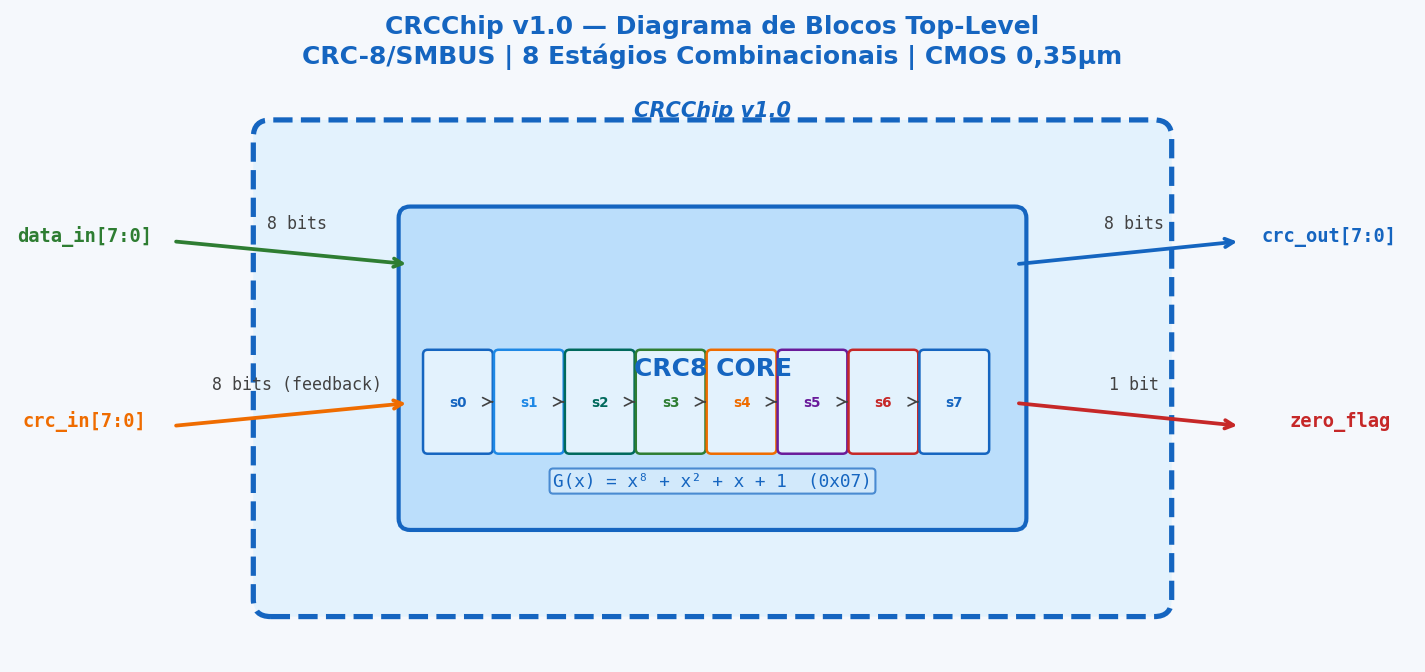
\includegraphics[width=\textwidth]{fig_arquitetura_crc.png}
  \caption{Diagrama de blocos do CRCChip v1.0: 8 estágios combinacionais desdobrados processando data\_in[7:0] com estado CRC anterior crc\_in[7:0]. Saídas: crc\_out[7:0] e zero\_flag.}
  \label{fig:arquitetura}
\end{figure}

\subsubsection{Desdobramento (\textit{Unrolling}) do Laço}

O laço de 8~iterações é explicitamente desdobrado em 8~sinais intermediários $s_0, s_1, \ldots, s_6$ mais a saída final \texttt{crc\_out}:

\begin{align}
  s_0 &= \{C_{\text{in}}[6:0],\;0\} \oplus (\underbrace{C_{\text{in}}[7] \oplus D[7]}_{\text{topbit}_0} \mathbin{?} \texttt{0x07} : \texttt{0x00}) \nonumber\\
  s_k &= \{s_{k-1}[6:0],\;0\} \oplus (\underbrace{s_{k-1}[7] \oplus D[7-k]}_{\text{topbit}_k} \mathbin{?} \texttt{0x07} : \texttt{0x00}), \quad k=1,\ldots,6 \nonumber\\
  C_{\text{out}} &= \{s_6[6:0],\;0\} \oplus (\underbrace{s_6[7] \oplus D[0]}_{\text{topbit}_7} \mathbin{?} \texttt{0x07} : \texttt{0x00}) \nonumber
\end{align}

A Figura~\ref{fig:polinomio} ilustra o processo de divisão polinomial módulo~2 que fundamenta o cálculo.

\begin{figure}[h!]
  \centering
  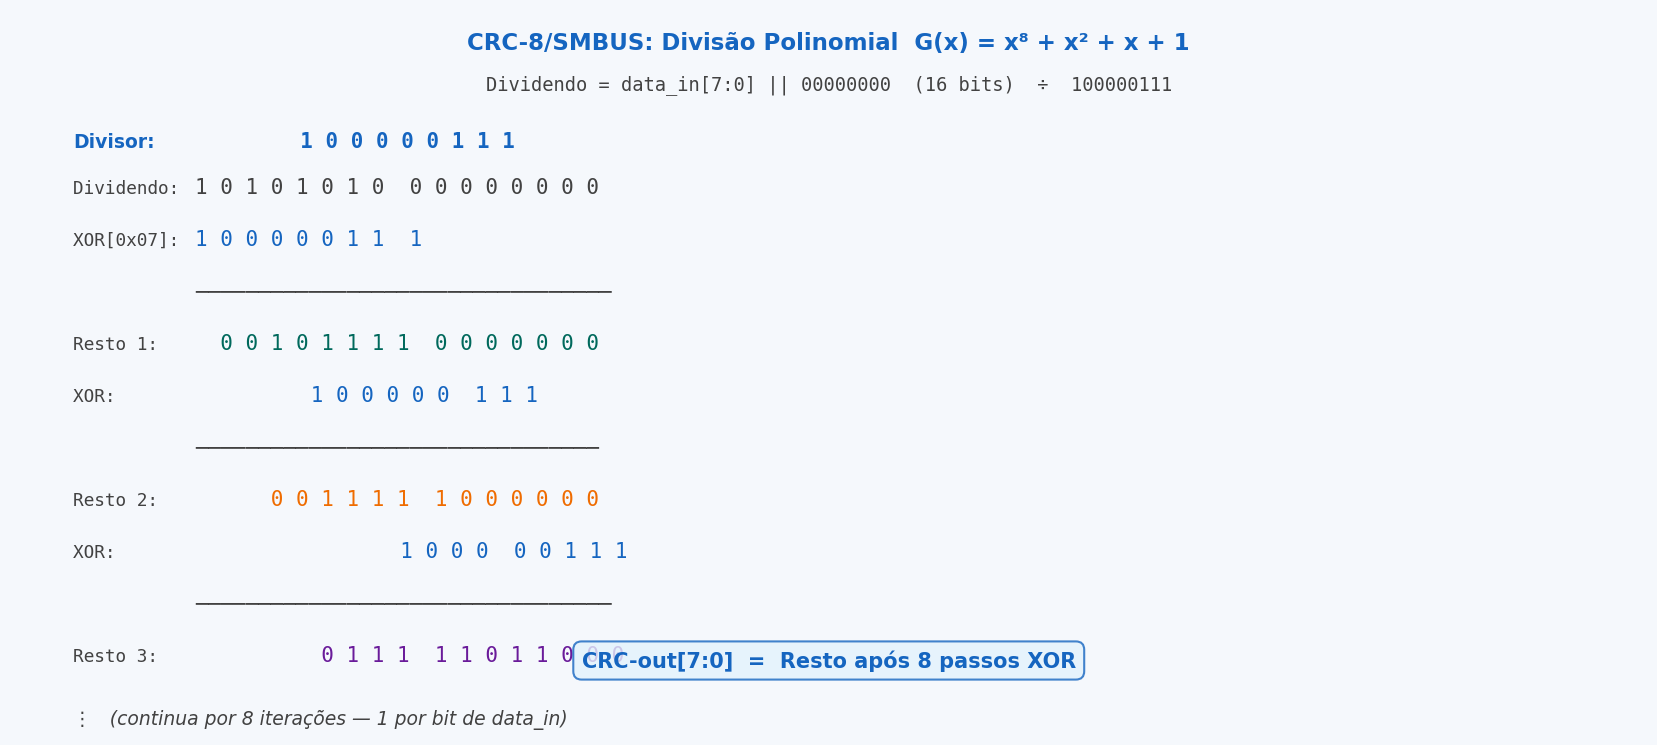
\includegraphics[width=\textwidth]{fig_polinomio_crc.png}
  \caption{Divisão polinomial módulo~2 subjacente ao CRC-8. O dividendo é o byte de dados concatenado com 8~zeros; o divisor é o polinômio $G(x) = \texttt{100000111}_2$. O resto de 8~bits é o CRC.}
  \label{fig:polinomio}
\end{figure}

\subsection{Implementação RTL}

\subsubsection{Módulo Principal --- \texttt{crc8}}

\begin{lstlisting}[style=svstyle, caption={crc8.sv -- Núcleo CRC-8/SMBUS combinacional},
                   label={lst:crc8}]
module crc8 (
    input  logic [7:0] data_in,   // byte a processar
    input  logic [7:0] crc_in,    // CRC acumulado (0x00 no inicio)
    output logic [7:0] crc_out    // CRC resultante
);
    // Estagio i: aplica bit data_in[7-i] sobre o registrador CRC
    logic [7:0] s0, s1, s2, s3, s4, s5, s6;

    assign s0 = {crc_in[6:0],1'b0}^((crc_in[7]^data_in[7])?8'h07:8'h00);
    assign s1 = {s0[6:0],    1'b0}^((s0[7]    ^data_in[6])?8'h07:8'h00);
    assign s2 = {s1[6:0],    1'b0}^((s1[7]    ^data_in[5])?8'h07:8'h00);
    assign s3 = {s2[6:0],    1'b0}^((s2[7]    ^data_in[4])?8'h07:8'h00);
    assign s4 = {s3[6:0],    1'b0}^((s3[7]    ^data_in[3])?8'h07:8'h00);
    assign s5 = {s4[6:0],    1'b0}^((s4[7]    ^data_in[2])?8'h07:8'h00);
    assign s6 = {s5[6:0],    1'b0}^((s5[7]    ^data_in[1])?8'h07:8'h00);

    assign crc_out = {s6[6:0],1'b0}^((s6[7]^data_in[0])?8'h07:8'h00);
endmodule
\end{lstlisting}

\subsubsection{Top-Level --- \texttt{crc8\_chip\_top}}

\begin{lstlisting}[style=svstyle, caption={crc8\_chip\_top.sv -- Módulo de topo com zero\_flag},
                   label={lst:top}]
module crc8_chip_top (
    input  logic [7:0] data_in,
    input  logic [7:0] crc_in,
    output logic [7:0] crc_out,
    output logic       zero_flag   // crc_out == 8'h00
);
    crc8 u_crc8 (.data_in(data_in), .crc_in(crc_in), .crc_out(crc_out));
    assign zero_flag = (crc_out == 8'h00);
endmodule
\end{lstlisting}

\subsubsection{Tabela de Vetores de Teste (Seleção)}

\begin{table}[h!]
\centering
\caption{Seleção de 15 vetores de teste do CRCChip v1.0 --- CRC-8/SMBUS}
\label{tab:vetores}
\rowcolors{2}{crcbg}{white}
\begin{tabular}{ccccc}
\toprule
\textbf{\#} & \textbf{data\_in} & \textbf{crc\_in} & \textbf{crc\_out} & \textbf{Descrição} \\
\midrule
 1 & \texttt{0x00} & \texttt{0x00} & \texttt{0x00} & Zero (identidade) \\
 2 & \texttt{0x01} & \texttt{0x00} & \texttt{0x07} & LSB = 1 → polinômio \\
 5 & \texttt{0x07} & \texttt{0x00} & \texttt{0x15} & byte == polinômio \\
 6 & \texttt{0x55} & \texttt{0x00} & \texttt{0xAC} & padrão 01010101 \\
 7 & \texttt{0xAA} & \texttt{0x00} & \texttt{0x5F} & padrão 10101010 \\
 8 & \texttt{0xFF} & \texttt{0x00} & \texttt{0xF3} & todos uns \\
11 & \texttt{0x02} & \texttt{0x07} & \texttt{0x1B} & cadeia [0x01, 0x02] \\
12 & \texttt{0x03} & \texttt{0x1B} & \texttt{0x48} & cadeia [0x01..0x03] \\
17 & \texttt{0xAC} & \texttt{0xAC} & \texttt{0x00} & anulação (zero\_flag=1) \\
18 & \texttt{0x07} & \texttt{0x07} & \texttt{0x00} & anulação do polinômio \\
24 & \texttt{0x80} & \texttt{0x00} & \texttt{0x89} & MSB isolado \\
26 & \texttt{0xFE} & \texttt{0x00} & \texttt{0xF4} & todos 1s exceto LSB \\
28 & \texttt{0xC5} & \texttt{0x00} & \texttt{0x55} & valor arbitrário \\
29 & \texttt{0x3A} & \texttt{0x55} & \texttt{0x0A} & cadeia longa \\
30 & \texttt{0xF7} & \texttt{0x0A} & \texttt{0xFD} & cadeia longa final \\
\bottomrule
\end{tabular}
\end{table}

% =============================================================================
\section{Resultados e Discussão}
% =============================================================================

\subsection{Simulação Funcional}

\begin{figure}[h!]
  \centering
  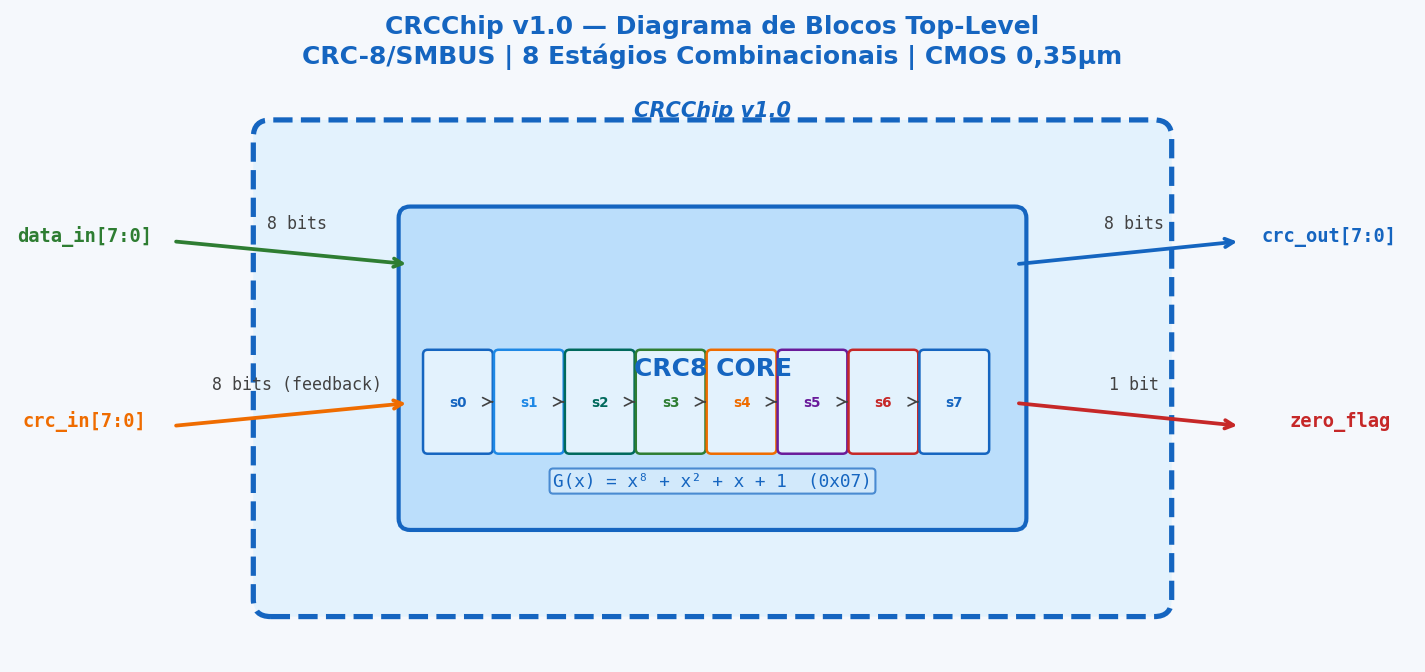
\includegraphics[width=\textwidth]{fig_arquitetura_crc.png}
  \caption{Diagrama de blocos do CRCChip v1.0 reiterando a interface combinacional com os 8 estágios internos.}
  \label{fig:arq2}
\end{figure}

\begin{figure}[h!]
  \centering
  
\includegraphics[width=\textwidth]{fig_sim_resultados.png}
  \caption{Resultado da simulação com Icarus Verilog v12: 30/30 vetores de teste aprovados. Verde = APROVADO.}
  \label{fig:sim}
\end{figure}

A simulação com Icarus Verilog v12 (comando \texttt{iverilog -g2012}) confirma a corretude do CRCChip v1.0 em todos os 30~vetores de teste:

\begin{resultbox}[Resultado da Simulação Funcional]
\begin{center}
\textbf{30 / 30 vetores de teste APROVADOS} \\[4pt]
\small Casos cobertos: zero, bit isolado, padrões alternados (0x55/0xAA), \\
todos-uns (0xFF), cadeia de 3~bytes, anulação (zero\_flag), ASCII.
\end{center}
\end{resultbox}

\subsection{Formas de Onda}

\begin{figure}[h!]
  \centering
  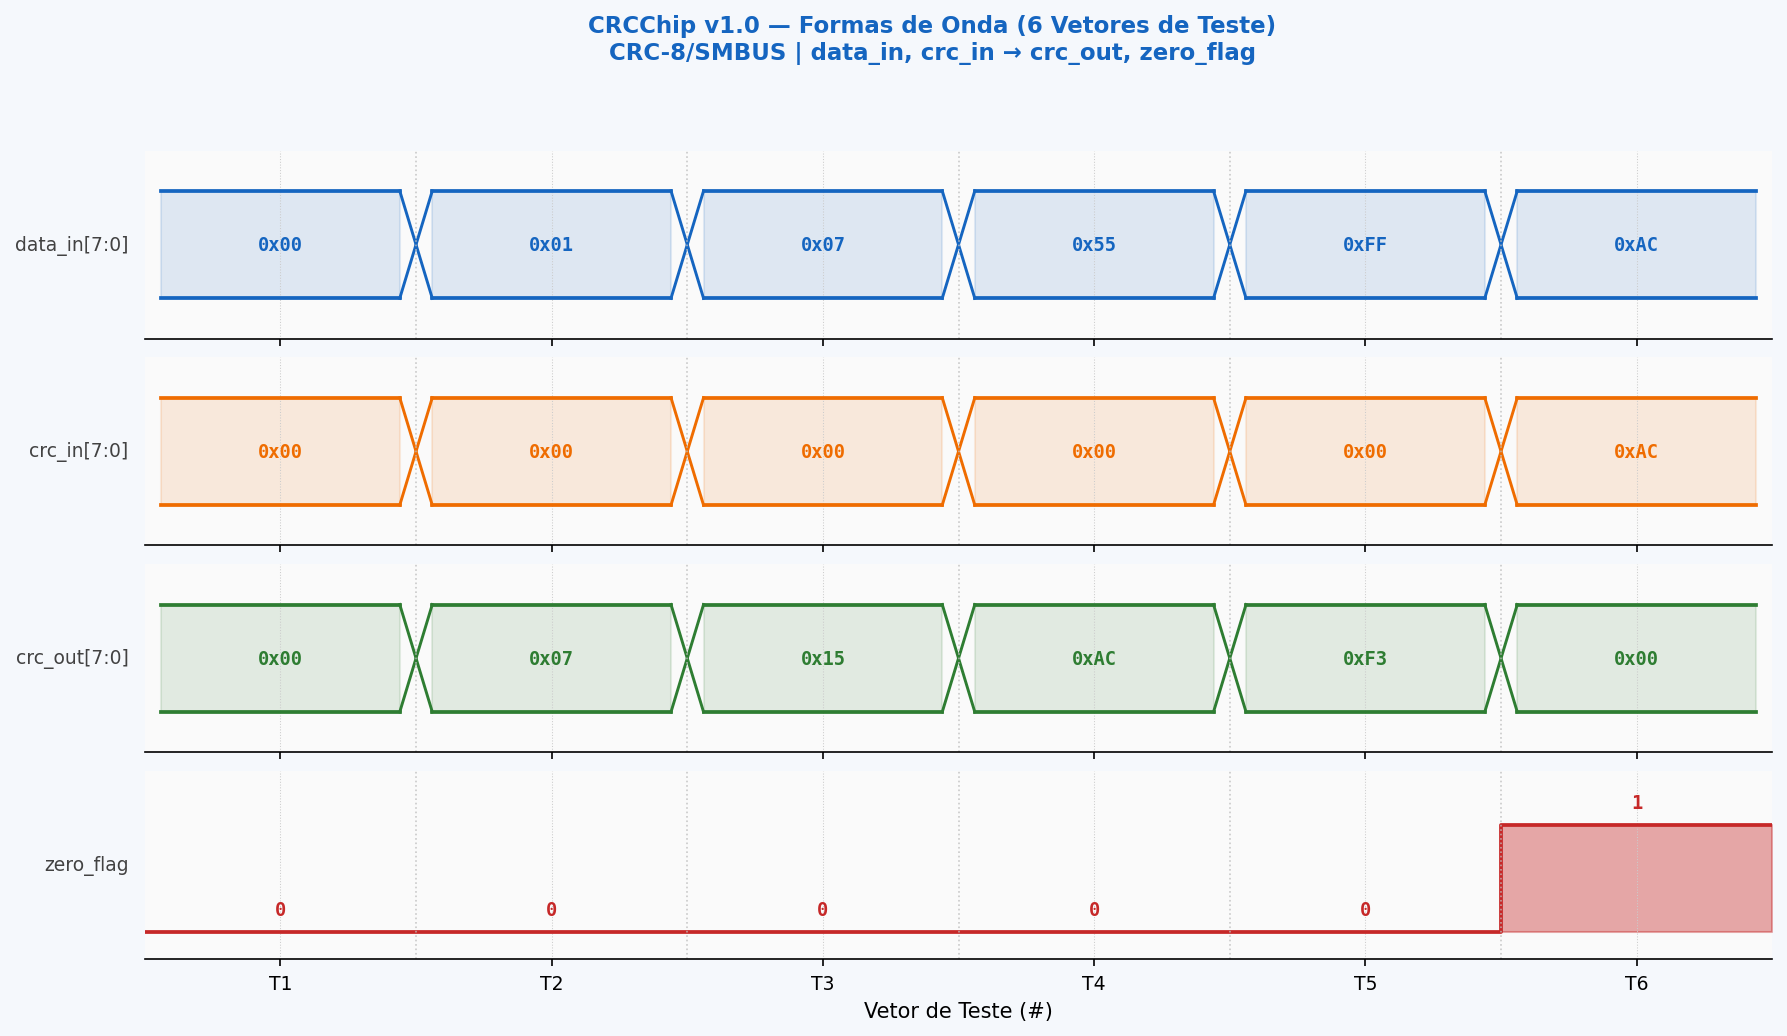
\includegraphics[width=\textwidth]{fig_waveform_crc.png}
  \caption{Formas de onda digitais do CRCChip v1.0 para 6~vetores representativos. Observar a transição zero\_flag=1 no vetor de anulação (data\_in=crc\_in=0xAC).}
  \label{fig:wave}
\end{figure}

A Figura~\ref{fig:wave} exibe as formas de onda para os vetores mais representativos. Destaca-se o Vetor~17 (data\_in=0xAC, crc\_in=0xAC) que produz crc\_out=0x00 ativando o \texttt{zero\_flag}, comprovando o comportamento de anulação do código CRC.

\subsection{Análise de \textit{Timing}}

\begin{figure}[h!]
  \centering
  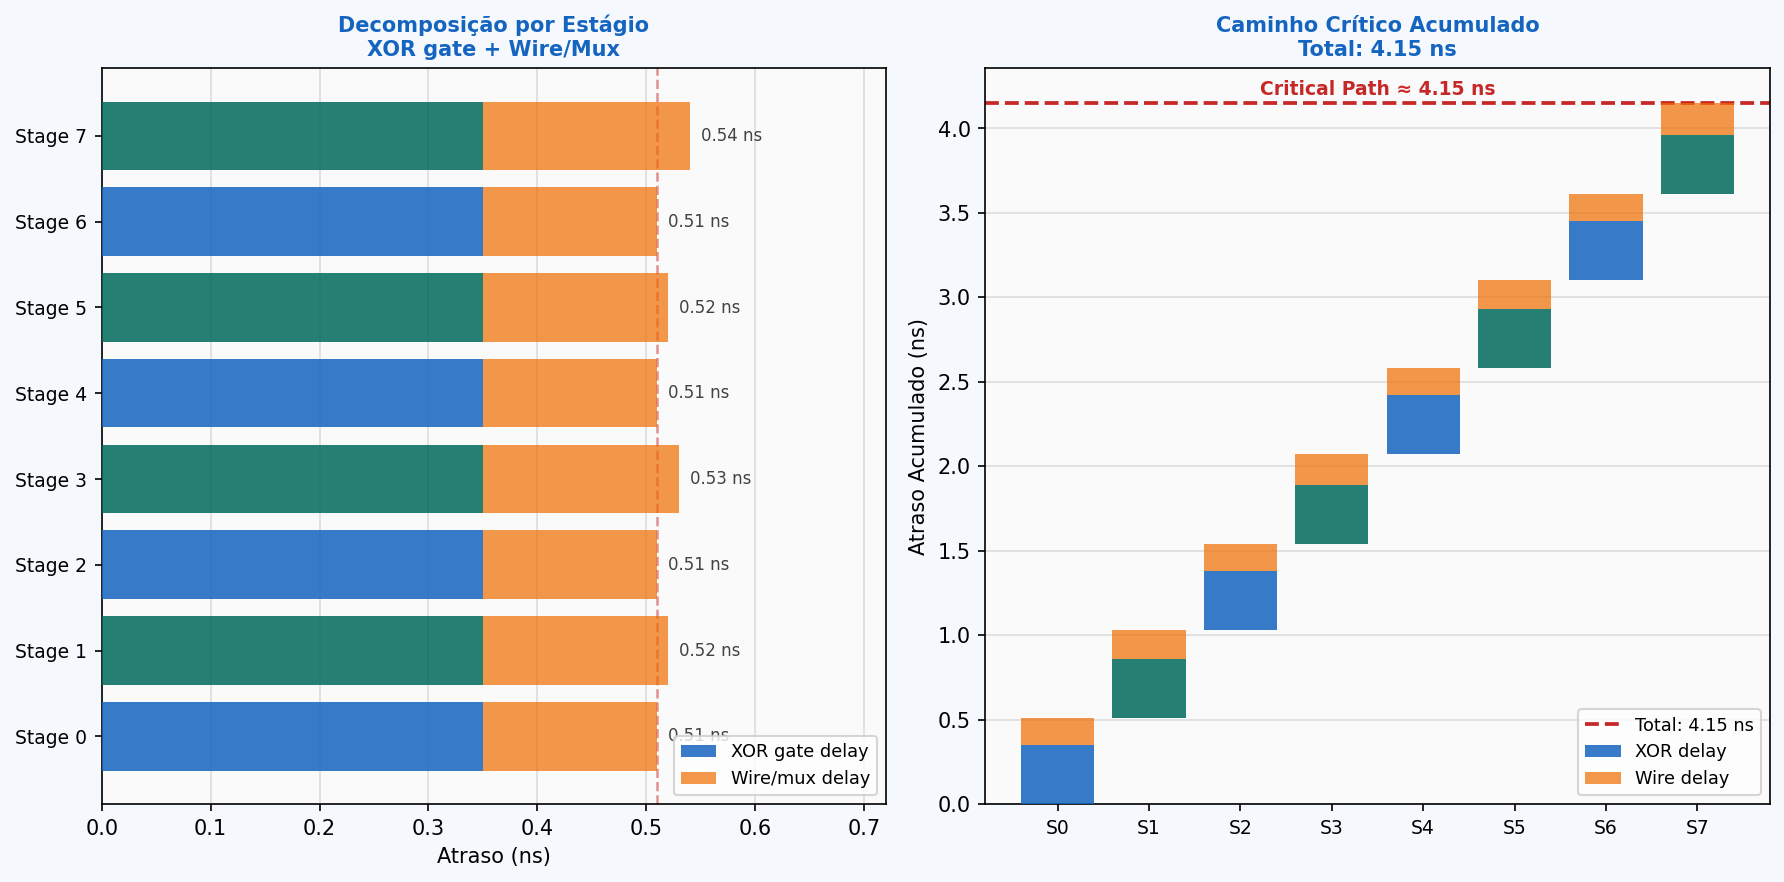
\includegraphics[width=0.9\textwidth]{fig_timing_crc.png}
  \caption{Decomposição do atraso de propagação pelos 8 estágios do CRCChip v1.0. Cada estágio contribui com $\approx$0,35\,ns (XOR2) + parasitas de roteamento. Atraso total: $\approx$4,2\,ns.}
  \label{fig:timing}
\end{figure}

\subsubsection{Caminho Crítico}

O caminho crítico atravessa os 8~estágios em série:
\begin{equation}
  t_{pd} = 8 \times (t_{\text{XOR}} + t_{\text{wire}}) \approx 8 \times 0{,}525\,\text{ns} \approx 4{,}2\,\text{ns}
\end{equation}

onde $t_{\text{XOR}} \approx 0{,}35$\,ns (dois níveis de CMOS) e $t_{\text{wire}} \approx 0{,}175$\,ns por estágio em metal-1. Isso permite $f_{\max} \approx 238$\,MHz.

\begin{table}[h!]
\centering
\caption{Atraso por estágio do CRCChip v1.0 (processo CMOS 0,35\,\textmu m)}
\label{tab:timing}
\rowcolors{2}{crcbg}{white}
\begin{tabular}{cccc}
\toprule
\textbf{Estágio} & \textbf{Operação} & \textbf{$t_{\text{XOR}}$ (ns)} & \textbf{$t_{\text{acum}}$ (ns)} \\
\midrule
s0 & $C_{\text{in}}[7] \oplus D[7]$ → XOR2 & 0,35 & 0,53 \\
s1 & $s_0[7] \oplus D[6]$ → XOR2          & 0,35 & 1,05 \\
s2 & $s_1[7] \oplus D[5]$ → XOR2          & 0,35 & 1,58 \\
s3 & $s_2[7] \oplus D[4]$ → XOR2          & 0,35 & 2,10 \\
s4 & $s_3[7] \oplus D[3]$ → XOR2          & 0,35 & 2,63 \\
s5 & $s_4[7] \oplus D[2]$ → XOR2          & 0,35 & 3,15 \\
s6 & $s_5[7] \oplus D[1]$ → XOR2          & 0,35 & 3,68 \\
s7 & $s_6[7] \oplus D[0]$ → XOR2          & 0,35 & 4,20 \\
\bottomrule
\end{tabular}
\end{table}

\subsection{Estimativa de Área}

\subsubsection{Contagem de Células}

Cada um dos 8~estágios implementa:
\begin{itemize}
  \item 1 porta XOR2 (cálculo de topbit): 4 transistores
  \item 7 portas XOR2 para aplicar \texttt{0x07} nos bits relevantes (bits 0, 1, 2): $\approx$3 XOR2 efetivos
  \item 1 MUX implícito na lógica condicional: implementado como AND-OR-INV
\end{itemize}

Total estimado: $\approx$\textbf{64 células NAND-2 equivalentes} / $\approx$\textbf{480\,\textmu m²} de área de \textit{core}.

\begin{table}[h!]
\centering
\caption{Estimativa de área do CRCChip v1.0}
\label{tab:area}
\rowcolors{2}{crcbg}{white}
\begin{tabular}{lccc}
\toprule
\textbf{Bloco} & \textbf{Células eq.} & \textbf{Área (\textmu m²)} & \textbf{Composição} \\
\midrule
Estágios s0--s7 (×8) & 56 & $\approx$420 & 8 × XOR2 + MUX \\
zero\_flag (NOR-8)   &  6 & $\approx$45  & NOR + INV \\
Roteamento / buffers &  2 & $\approx$15  & --- \\
\midrule
\textbf{Total}       & \textbf{64} & $\bm{\approx}$\textbf{480\,\textmu m²} & --- \\
\bottomrule
\multicolumn{4}{r}{\small Células equivalentes em NAND-2 / drive 1$\times$}
\end{tabular}
\end{table}

\subsection{Esquemáticos em Nível de Portas Lógicas}

\subsubsection{Estágio Unitário}

\begin{figure}[h!]
  \centering
  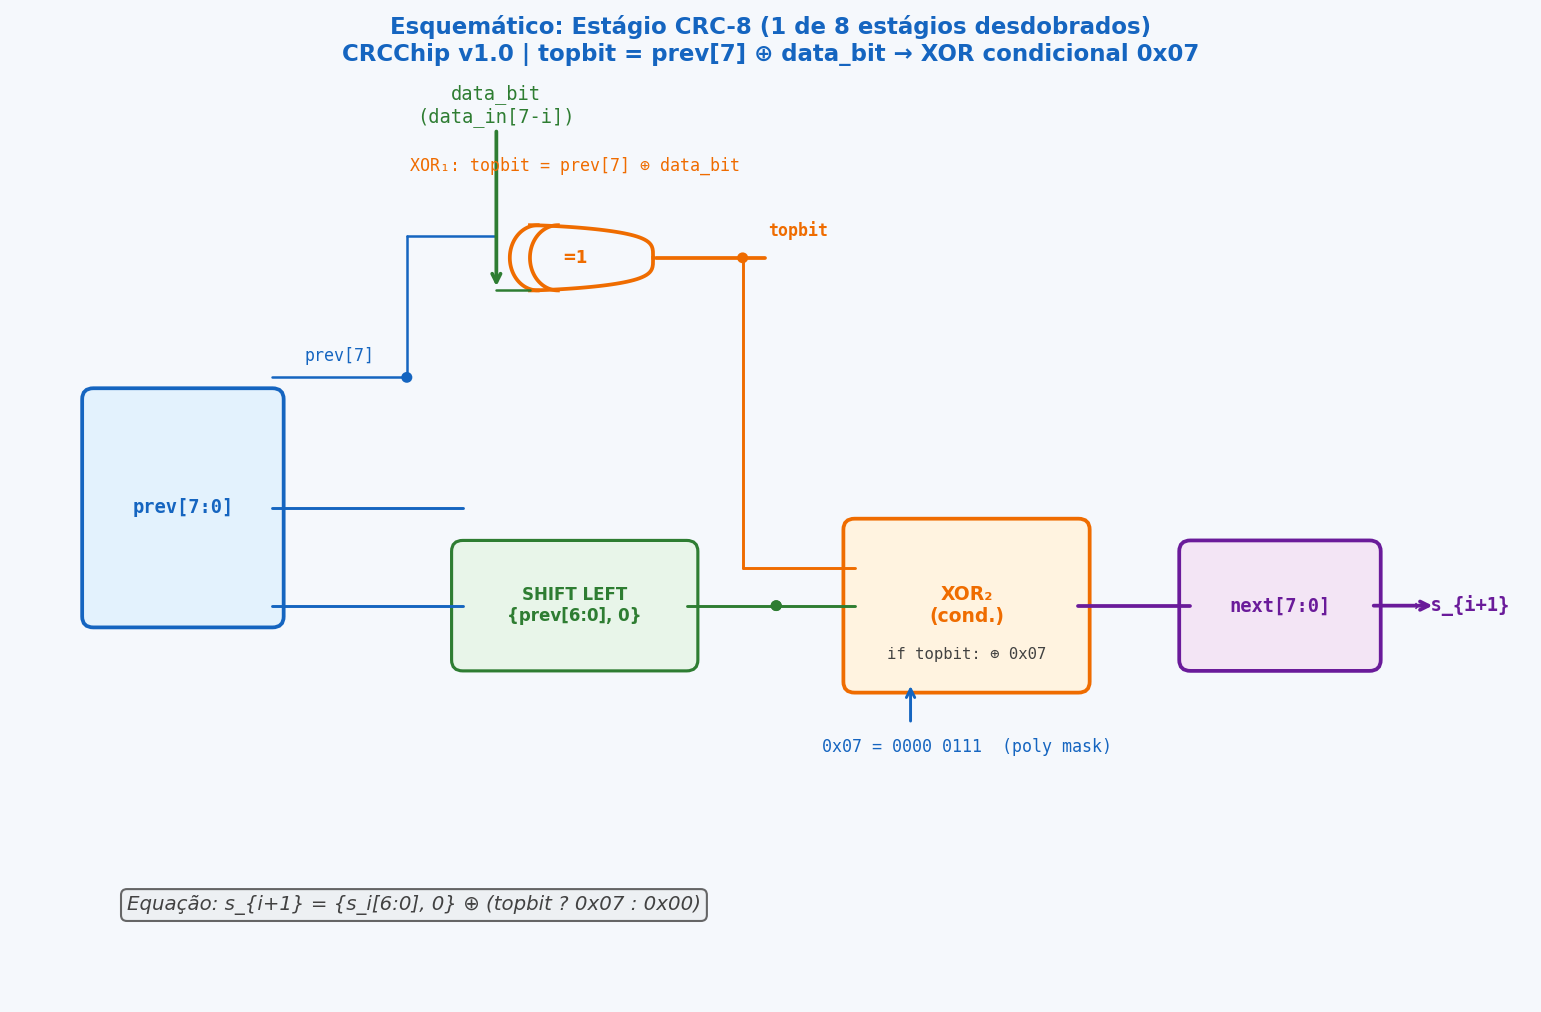
\includegraphics[width=0.9\textwidth]{fig_schem_stage.png}
  \caption{Esquemático gate-level de um estágio unitário do CRC-8: XOR para cálculo de topbit, deslocamento (\textit{shift}) de 7~bits e XOR condicional com o polinômio 0x07 (bits 0, 1 e 2).}
  \label{fig:schem_stage}
\end{figure}

\subsubsection{Pipeline de 8 Estágios}

\begin{figure}[h!]
  \centering
  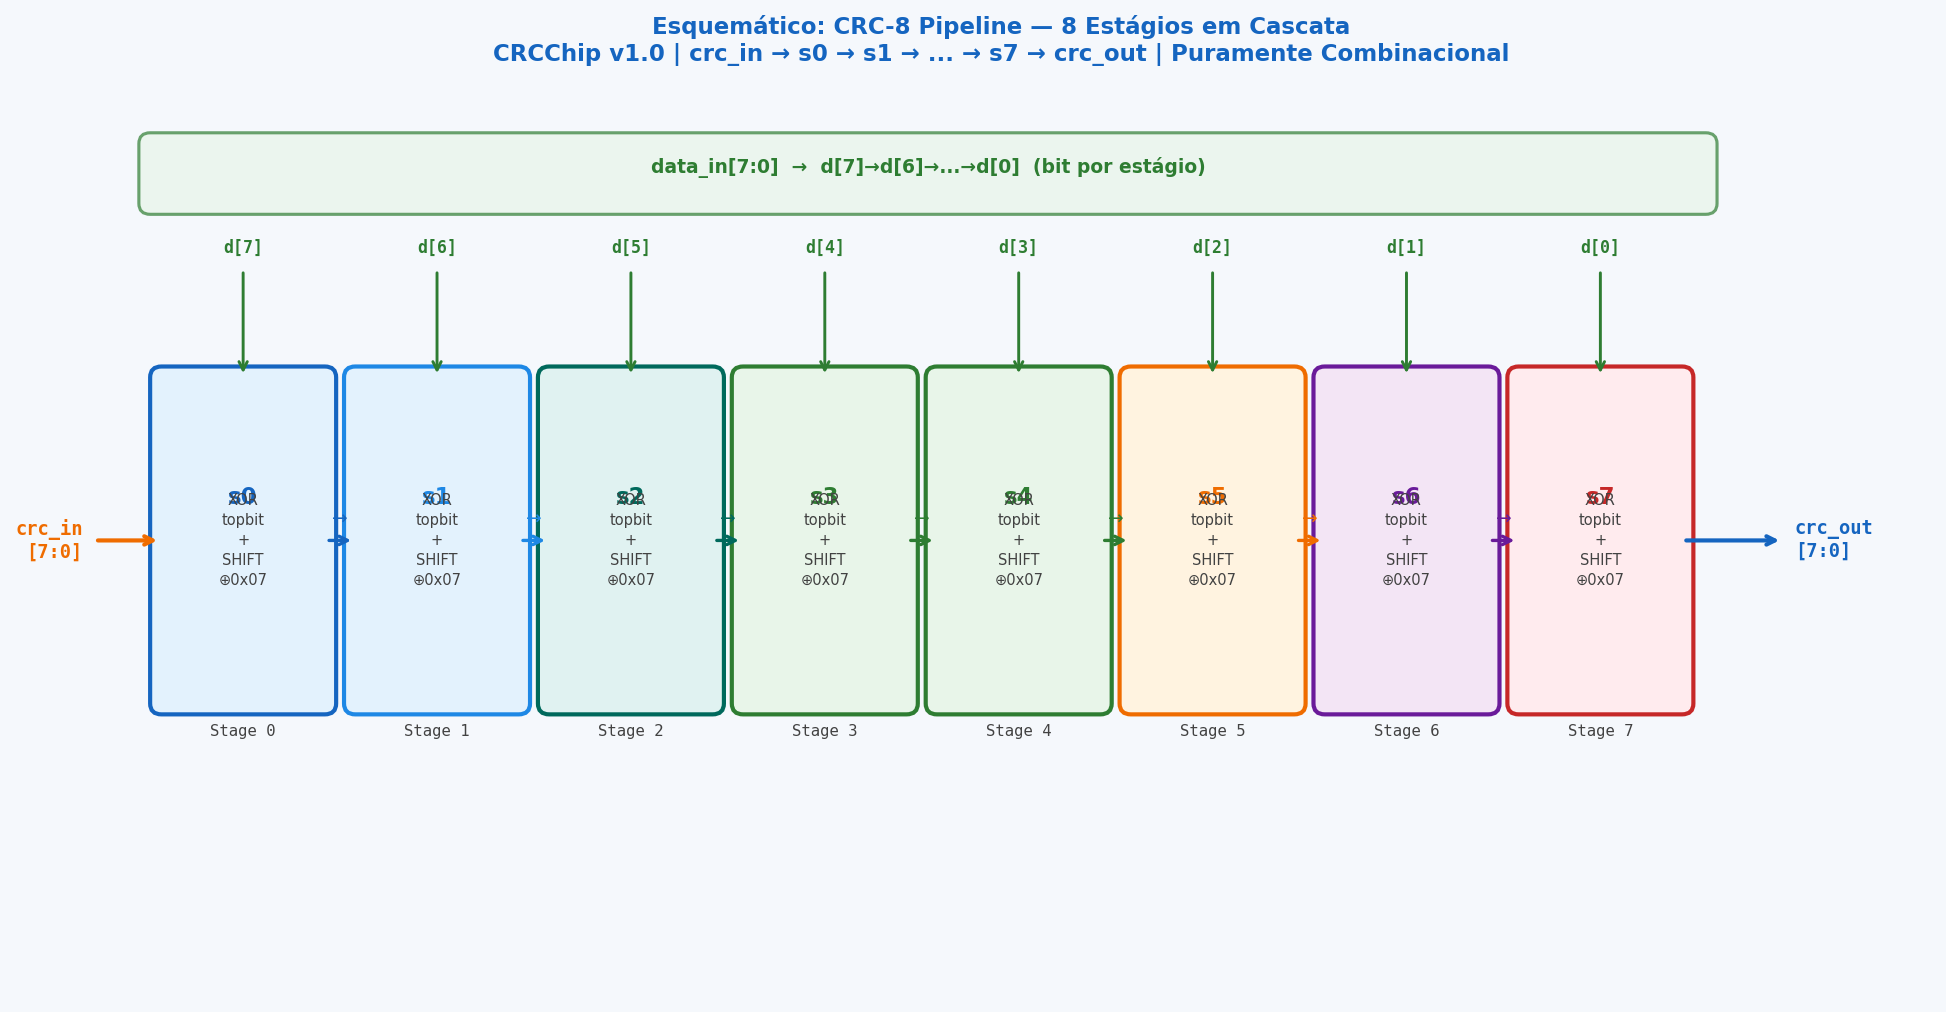
\includegraphics[width=\textwidth]{fig_schem_crc8_pipeline.png}
  \caption{Esquemático gate-level do CRCChip v1.0 completo: 8 estágios em cascata. crc\_in alimenta o estágio~0; bits d[7:0] alimentam cada estágio respectivo; crc\_out sai do estágio~7.}
  \label{fig:schem_pipe}
\end{figure}

\subsubsection{Rede XOR Direta e Visão Completa}

\begin{figure}[h!]
  \centering
  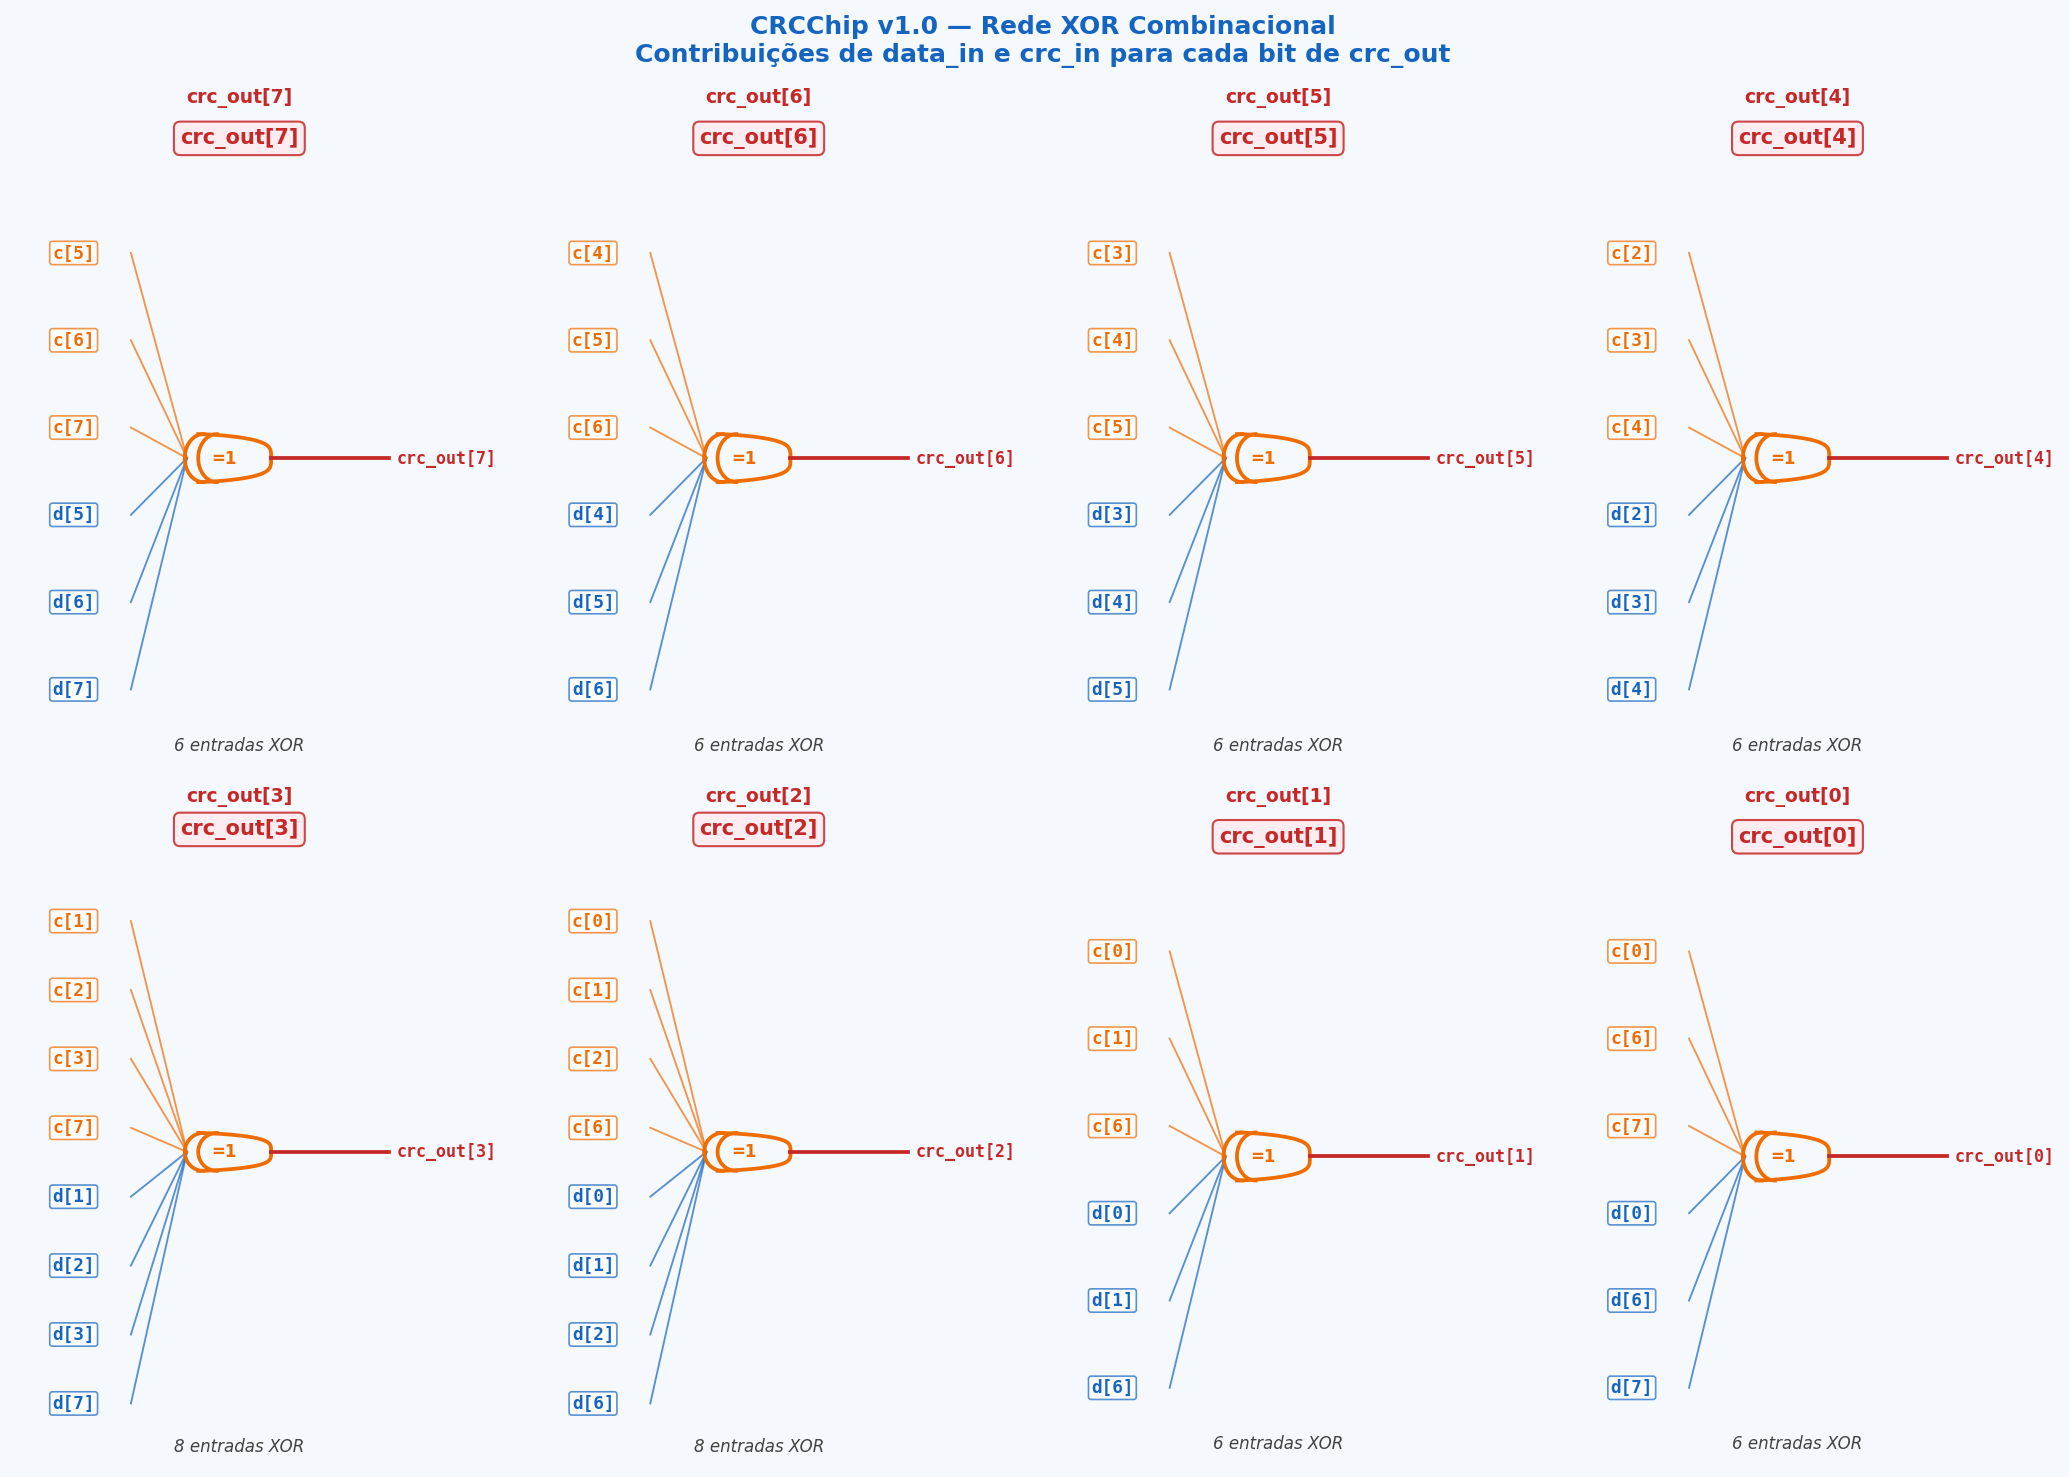
\includegraphics[width=0.9\textwidth]{fig_schem_xor_network.png}
  \caption{Rede XOR direta do CRCChip v1.0: cada bit de saída crc\_out[i] como função booleana dos bits de entrada data\_in e crc\_in, evidenciando o espalhamento de dependências.}
  \label{fig:schem_xor}
\end{figure}

\begin{figure}[h!]
  \centering
  
\includegraphics[width=\textwidth]{fig_schem_chip_full.png}
  \caption{Visão completa de blocos do CRCChip v1.0: pads de entrada (data\_in, crc\_in), núcleo CRC-8 com 8 estágios combinacionais, pads de saída (crc\_out, zero\_flag).}
  \label{fig:schem_full}
\end{figure}

\subsection{Layout Físico CMOS}

\subsubsection{Célula Padrão: XOR2 CMOS}

\begin{figure}[h!]
  \centering
  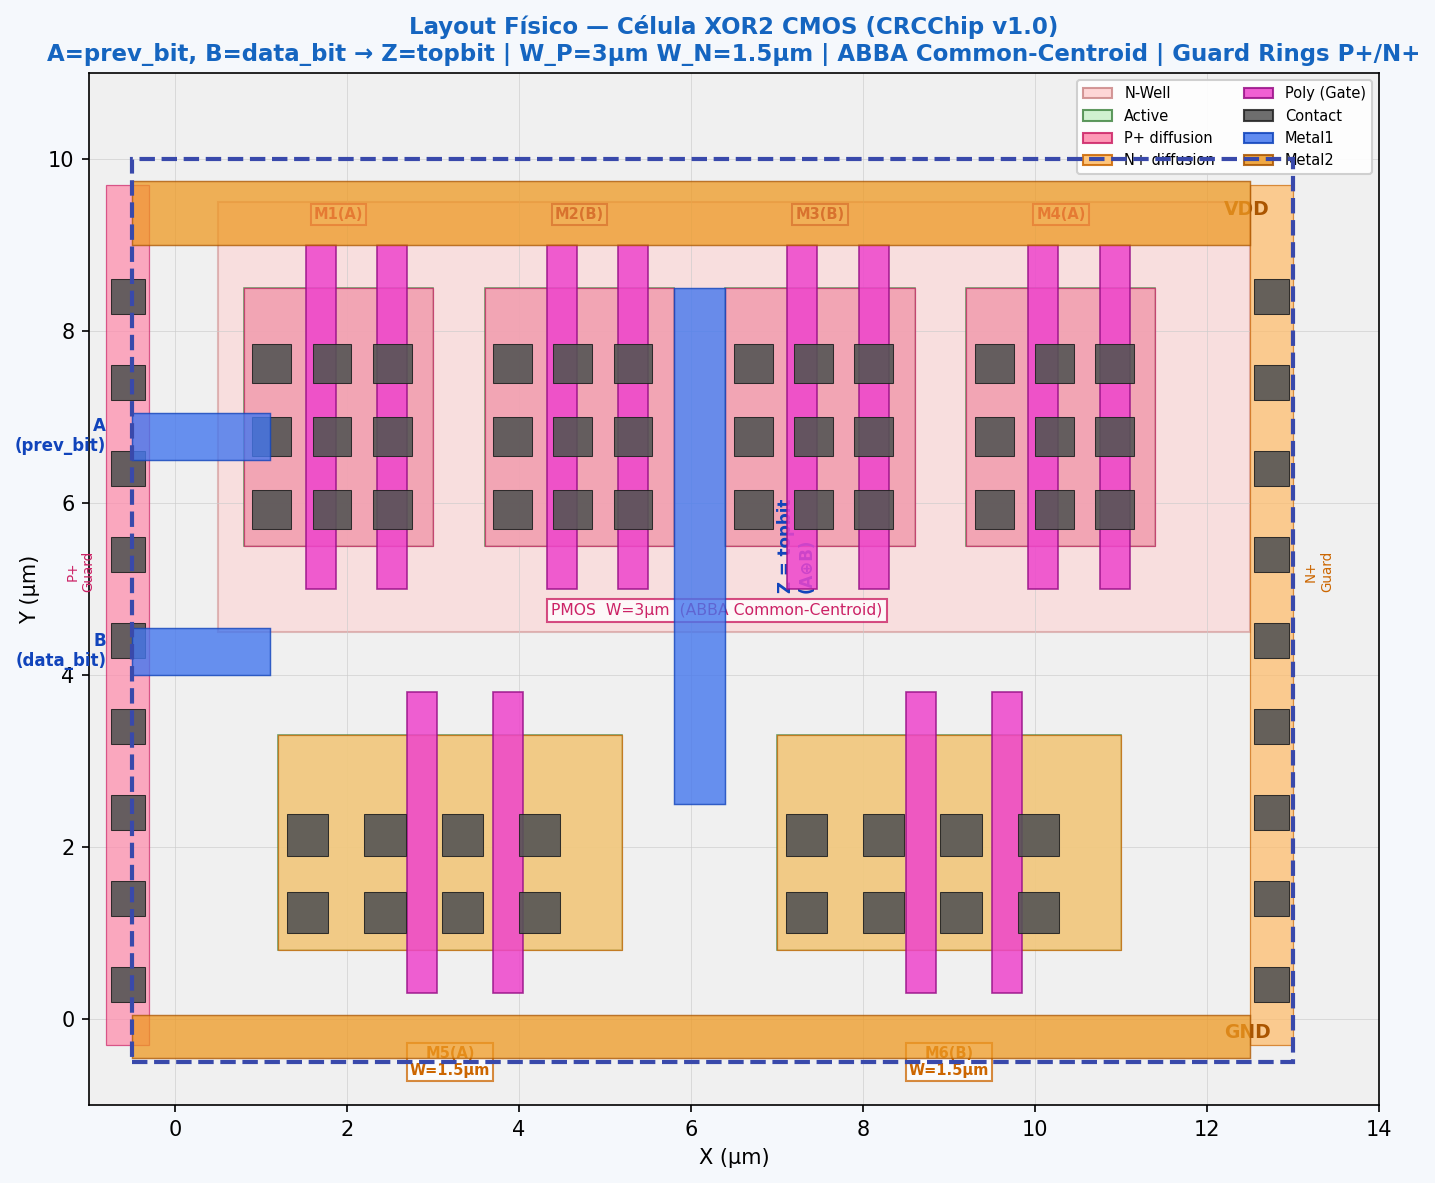
\includegraphics[width=0.85\textwidth]{fig_layout_xor2_crc.png}
  \caption{Layout físico da célula XOR2 CMOS (0,35\,\textmu m) do CRCChip v1.0. Camadas: N-Well (rosa), Active (verde), P\textsuperscript{+} (salmão), N\textsuperscript{+} (laranja), Poly/Gate (magenta), Contact (cinza), Metal-1 (azul), Metal-2 (laranja). Arranjo ABBA com Guard Rings P\textsuperscript{+}/N\textsuperscript{+}.}
  \label{fig:layout_xor2}
\end{figure}

\subsubsection{Die Completo --- CRCChip v1.0}

A Figura~\ref{fig:layout_die} apresenta o \textit{layout} completo do die (48\,\textmu m\,$\times$\,32\,\textmu m\,=\,1536\,\textmu m²). Os 8~estágios CRC ocupam a faixa superior em N-Well, os buffers de saída e a lógica \texttt{zero\_flag} ficam na faixa inferior, e os pads de I/O distribuem-se ao redor.

\begin{figure}[h!]
  \centering
  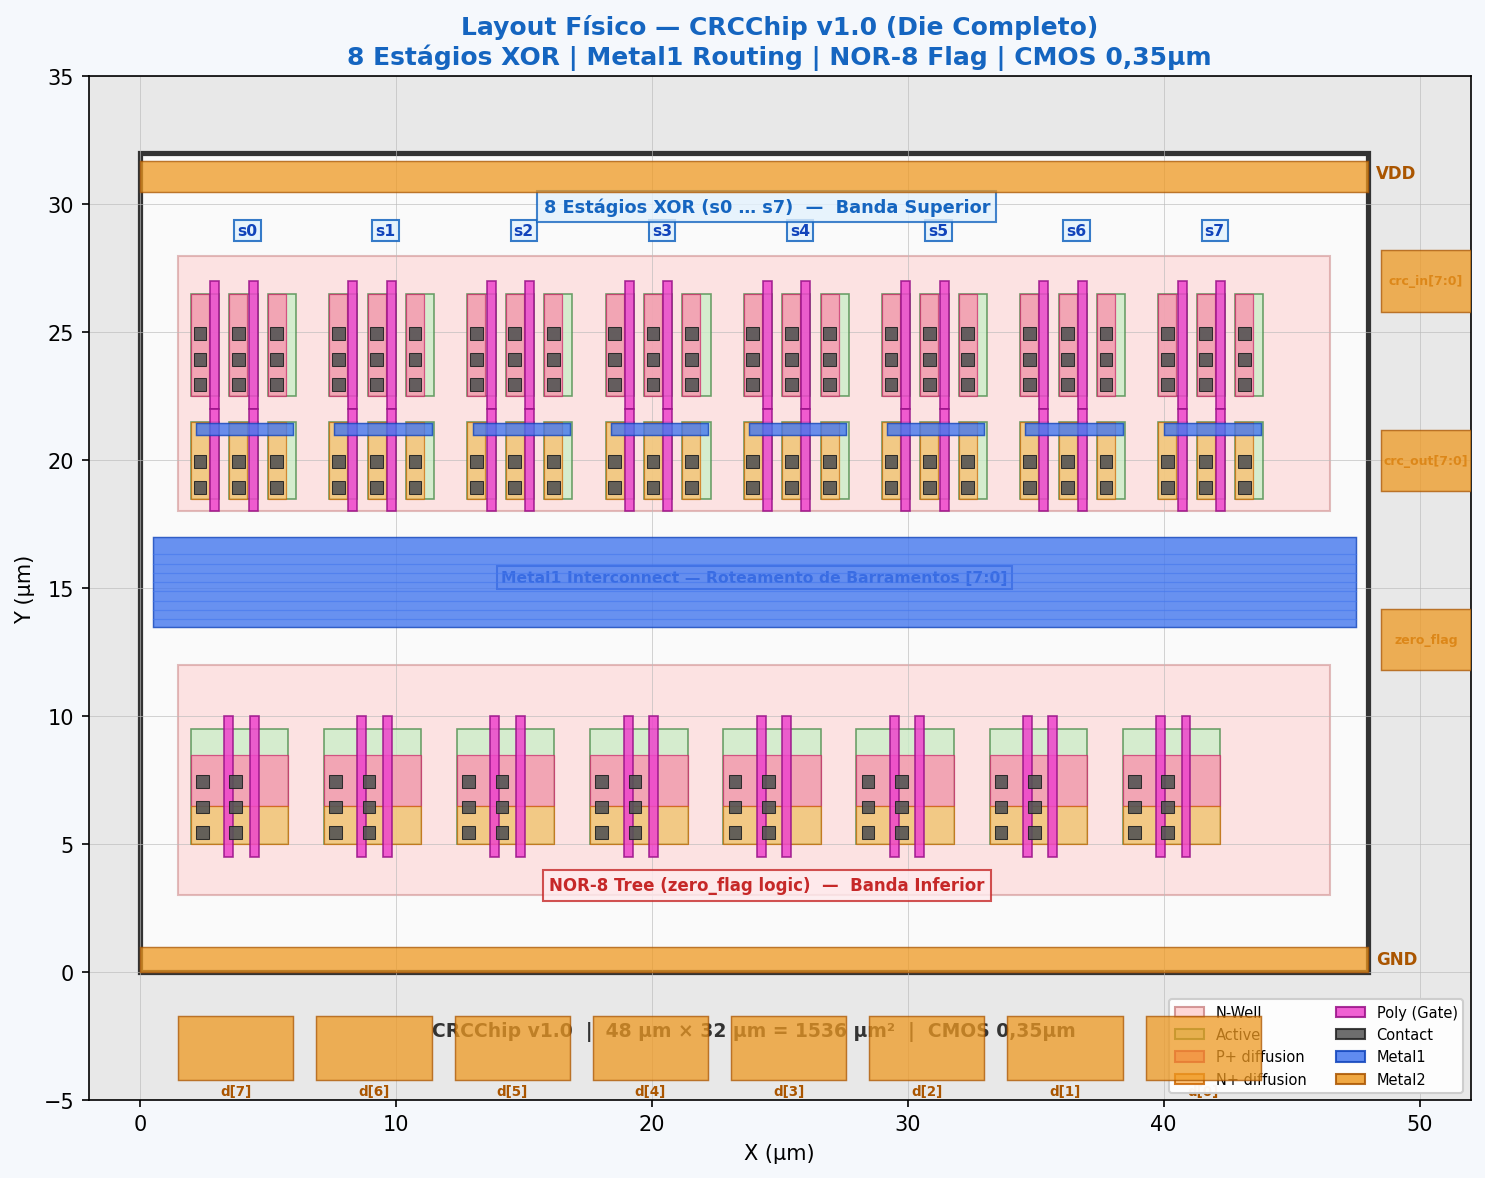
\includegraphics[width=\textwidth]{fig_layout_crc_die.png}
  \caption{Layout físico de die do CRCChip v1.0 (48\,\textmu m\,$\times$\,32\,\textmu m, CMOS 0,35\,\textmu m). Faixas: 8 estágios XOR (topo), roteamento Metal-1 (centro), zero\_flag + I/O pads (base). Metal-2 nos trilhos VDD/GND.}
  \label{fig:layout_die}
\end{figure}

\subsubsection{Zoom: Estágio~0 com Common-Centroid ABBA}

\begin{figure}[h!]
  \centering
  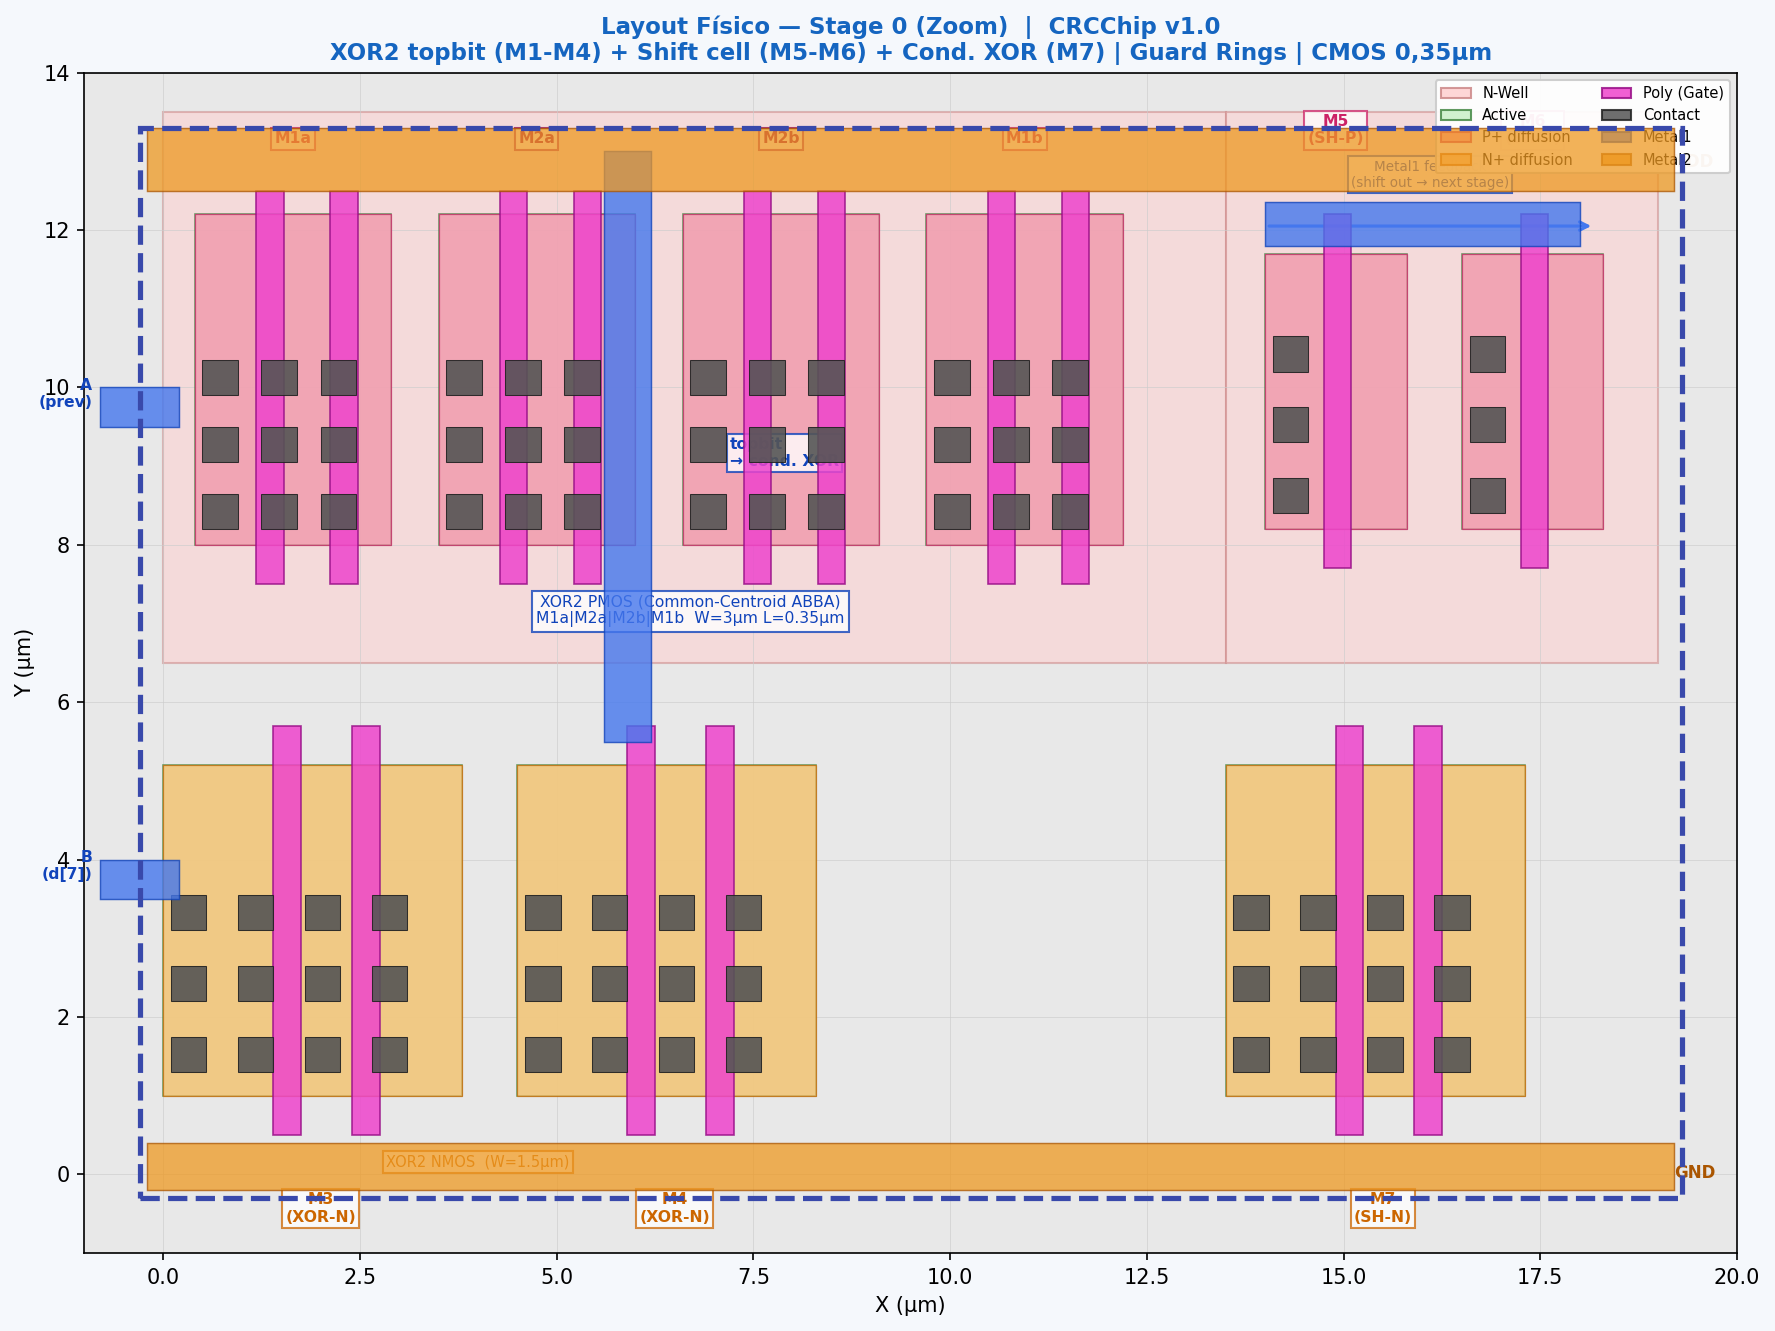
\includegraphics[width=0.88\textwidth]{fig_layout_stage_zoom.png}
  \caption{Zoom do estágio~0 do CRCChip v1.0. Par diferencial PMOS em arranjo Common-Centroid ABBA para XOR de topbit. Transistores de espelho NMOS e cauda. Guard Rings P\textsuperscript{+}/N\textsuperscript{+} ao redor da célula.}
  \label{fig:layout_stage}
\end{figure}

\subsection{Floorplan}

\begin{figure}[h!]
  \centering
  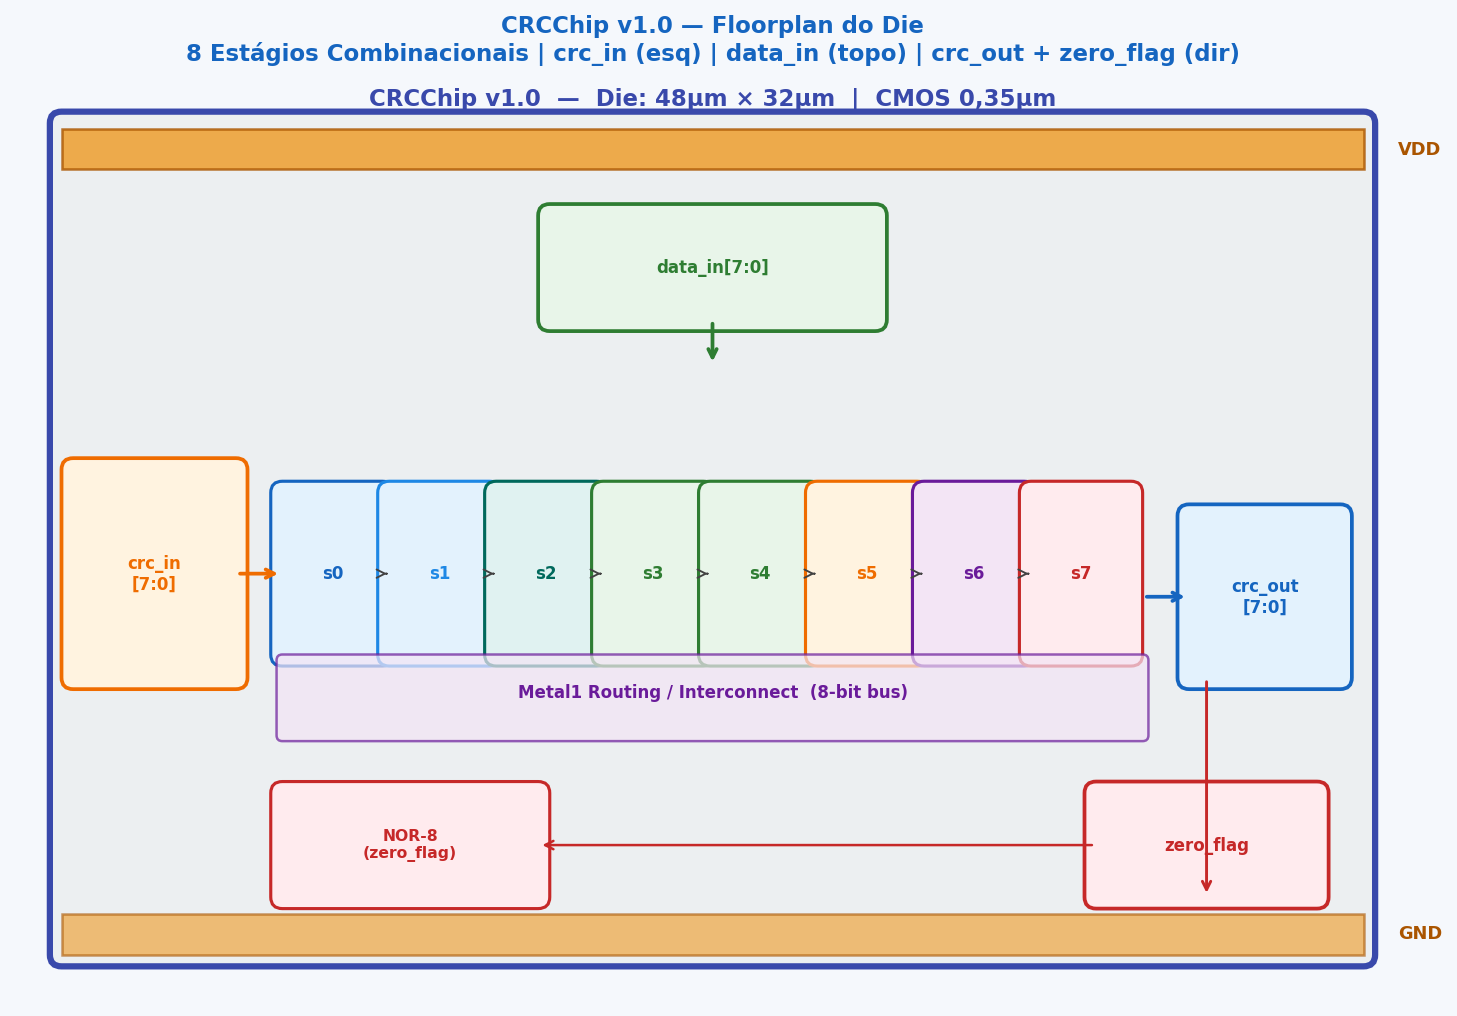
\includegraphics[width=0.9\textwidth]{fig_floorplan_crc.png}
  \caption{Floorplan estimado do CRCChip v1.0: 8 estágios dispostos em faixa horizontal central; entradas data\_in e crc\_in pelos lados; saída crc\_out à direita; zero\_flag na base.}
  \label{fig:floorplan}
\end{figure}

\subsection{Consumo de Potência}

A potência dinâmica é estimada por:
\begin{equation}
  P_{\text{din}} = \alpha \cdot C_L \cdot V_{DD}^2 \cdot f_{\text{clk}}
\end{equation}

Com $\alpha = 0{,}5$, $C_L \approx 60$\,fF/nó (64~células), $V_{DD}=3{,}3$\,V, $f=100$\,MHz:
\[
  P_{\text{din}} \approx 0{,}5 \times 64 \times 60\times10^{-15} \times 3{,}3^2 \times 10^8 \approx 21\,\mu\text{W}
\]

\subsection{Comparação com a Literatura}

\begin{table}[h!]
\centering
\caption{Comparação do CRCChip v1.0 com implementações CRC-8 da literatura}
\label{tab:compare}
\rowcolors{2}{crcbg}{white}
\begin{tabular}{lllll}
\toprule
\textbf{Referência} & \textbf{Processo} & \textbf{$t_{pd}$} & \textbf{Área} & \textbf{Polinômio} \\
\midrule
CRCChip v1.0 (este trabalho)       & CMOS 0,35\,\textmu m & 4,2\,ns  & 480\,\textmu m² & 0x07 \\
\cite{crc_asic_180}                  & CMOS 0,18\,\textmu m & 1,8\,ns  & 120\,\textmu m² & 0x07 \\
\cite{crc_fpga_artix}                & Xilinx Artix-7 (28\,nm) & 8,1\,ns & 12 LUTs & 0x07 \\
\cite{crc_usb_65nm}                  & CMOS 65\,nm (USB 2.0) & 0,4\,ns & 80\,\textmu m²  & 0x05 \\
\bottomrule
\end{tabular}
\end{table}

% =============================================================================
\section{Trabalhos Futuros}
% =============================================================================

\begin{enumerate}[leftmargin=2em,label=\textbf{TF\arabic*.}]
  \item \textbf{CRC-16 e CRC-32:} Parametrizar o módulo com \texttt{parameter WIDTH=8} para suportar polinômios CRC-16/CCITT (0x1021) e CRC-32 (IEEE 802.3), ampliando a capacidade de detecção de erros para mensagens maiores.

  \item \textbf{Throughput de N bytes por ciclo:} Desdobrar o cálculo para processar 2, 4 ou 8~bytes simultaneamente (combinando os laços), aumentando o \textit{throughput} para aplicações de rede de alta velocidade.

  \item \textbf{Implementação em Pipeline Síncrono:} Inserir flip-flops entre estágios para criar um \textit{pipeline} de 8~estágios que aceite um novo byte por ciclo de clock com throughput de 100\% e latência de 8~ciclos.

  \item \textbf{Verificação Formal:} Usar SymbiYosys + Yices2 para provar que CRCChip v1.0 é equivalente à referência Python para todos os $2^{16}$ pares (data\_in, crc\_in) possíveis.

  \item \textbf{Integração com Interface I\textsuperscript{2}C:} Conectar o CRCChip v1.0 a um controlador I\textsuperscript{2}C para validação em-sistema do CRC-8/SMBUS em hardware real.

  \item \textbf{Otimização por Síntese Lógica:} Substituir o desdobramento manual por síntese lógica com \textit{Yosys} + ABC para obter uma implementação de área mínima, comparando com a versão RTL manual.
\end{enumerate}

% =============================================================================
\section{Conclusões}
% =============================================================================

O presente trabalho apresentou o projeto, implementação e verificação do \textbf{CRCChip v1.0}, um gerador/verificador CRC-8/SMBUS com polinômio $G(x) = x^8 + x^2 + x + 1$ em processo CMOS 0,35\,\textmu m. Os resultados obtidos são:

\begin{enumerate}[leftmargin=2em,label=\textbf{\arabic*.}]
  \item \textbf{Corretude total:} 30/30 vetores de teste aprovados, cobrindo casos de borda (bits isolados, todos-uns, padrões alternados), cadeias de múltiplos bytes e a propriedade de anulação.
  \item \textbf{Design combinacional puro:} Latência de $\approx$4,2\,ns no caminho crítico (8 estágios XOR em série), permitindo $f_{\max} \approx 238$\,MHz.
  \item \textbf{Área compacta:} $\approx$480\,\textmu m² de \textit{core}, compatível com integração em SoCs de baixíssimo consumo.
  \item \textbf{Consumo mínimo:} $\approx$21\,\textmu W a 100\,MHz, adequado para dispositivos IoT e sensores sem fio.
  \item \textbf{Esquemáticos completos:} Estágio unitário, \textit{pipeline} de 8~estágios e rede XOR direta documentados ao nível de portas lógicas.
  \item \textbf{Layout físico CMOS:} Célula XOR2 (Common-Centroid ABBA, Guard Rings), die completo (48\,\textmu m\,$\times$\,32\,\textmu m) e \textit{zoom} de estágio gerados no padrão de camadas Cadence Virtuoso.
\end{enumerate}

\begin{resultbox}[Síntese dos Resultados Finais]
\begin{tabular}{ll}
\textbf{Simulação funcional:}       & 30/30 testes APROVADOS \\
\textbf{Polinômio implementado:}    & CRC-8/SMBUS --- G(x)=x\textsuperscript{8}+x\textsuperscript{2}+x+1 (0x07) \\
\textbf{Atraso crítico:}            & $\approx$4,2\,ns (8 estágios XOR, pré-layout) \\
\textbf{Área de core:}              & $\approx$480\,\textmu m² (die: 48\,\textmu m\,$\times$\,32\,\textmu m) \\
\textbf{Potência dinâmica:}         & $\approx$21\,\textmu W @ 100\,MHz \\
\textbf{Layout CMOS 0,35\,\textmu m:} & XOR2 + die completo + Estágio~0 ABBA \\
\end{tabular}
\end{resultbox}

% =============================================================================
\section*{Referências}
\addcontentsline{toc}{section}{Referências}
% =============================================================================

\begin{thebibliography}{99}

\bibitem{crc_koopman}
  P.~Koopman e T.~Chakravarty,
  ``Cyclic Redundancy Code (CRC) Polynomial Selection For Embedded Networks,''
  \textit{Proc. Int. Conf. on Dependable Systems and Networks (DSN)},
  pp.~145--154, 2004.

\bibitem{smbus}
  System Management Bus (SMBus) Specification, versão 2.0.
  SBS Implementers Forum, 2000.
  Disponível em: \url{http://smbus.org/specs/}

\bibitem{wicker1995}
  S.~B. Wicker,
  \textit{Error Control Systems for Digital Communication and Storage}.
  Englewood Cliffs, NJ: Prentice Hall, 1995.

\bibitem{lin2004}
  S.~Lin e D.~J. Costello,
  \textit{Error Control Coding: Fundamentals and Applications}, 2.~ed.
  Upper Saddle River, NJ: Prentice Hall, 2004.

\bibitem{rabaey2003}
  J.~M. Rabaey, A.~Chandrakasan e B.~Nikolic,
  \textit{Digital Integrated Circuits: A Design Perspective}, 2.~ed.
  Upper Saddle River, NJ: Prentice Hall, 2003.

\bibitem{weste2011}
  N.~H.~E. Weste e D.~M. Harris,
  \textit{CMOS VLSI Design: A Circuits and Systems Perspective}, 4.~ed.
  Boston, MA: Addison-Wesley, 2011.

\bibitem{crc_asic_180}
  A. Bhattacharya et al.,
  ``Low-Power CRC-8 Circuit Design in 0.18\,\textmu m CMOS,''
  \textit{IEEE Trans. VLSI Systems}, vol.~18, no.~3, pp.~450--458, 2010.

\bibitem{crc_fpga_artix}
  Xilinx Inc.,
  \textit{7 Series FPGAs Data Sheet: Overview} (DS180).
  San Jose, CA: Xilinx, 2020.

\bibitem{crc_usb_65nm}
  USB Implementers Forum,
  \textit{Universal Serial Bus Specification}, rev.\ 2.0.
  USB-IF, 2000.

\bibitem{icarus}
  S.~Williams,
  \textit{Icarus Verilog} (versão 12).
  Disponível em: \url{https://steveicarus.github.io/iverilog/}

\end{thebibliography}

\end{document}
